% Source-derived chapter 01: Introduction
% Original source: refined-brill-noether-theory-hurwitz-spaces
\chapter{Introduction}
\label{refined-brill-noether-theory-hurwitz-spaces-chapter-01}
\source{refined-brill-noether-theory-hurwitz-spaces}

\begin{remark}[Source section]
\label{refined-brill-noether-theory-hurwitz-spaces-chapter-01-source}
\source{refined-brill-noether-theory-hurwitz-spaces}
\source{refined-brill-noether-theory-hurwitz-spaces}
This chapter reproduces the corresponding section of the retrieved
LaTeX source, including its definitions, statements, examples, and
proofs. It has not yet been translated into Lean.
\notready
\end{remark}

% The source section title was: Introduction
Brill-Noether theory characterizes the maps of general curves to projective space. 
Degree $d$ maps of a curve $C \rightarrow \pp^r$ correspond to line bundles in the \textit{Brill-Noether locus}
\[W^r_d(C) = \{ L \in \Pic^d(C): h^0(C, L) \geq r+1\}.\] 
The fundamental Brill-Noether-Petri theorem \cite{GH,G} states that for a general curve $C$ of genus $g$, 
\[\dim W^r_d(C) = \rho(g, r, d) := g - (r+1)(g - d + r),\]
and $W^r_d(C)$ is smooth away from $W^{r+1}_d(C)$. Furthermore, if $\rho(g, r, d) > 0$, then $W^r_d(C)$ is irreducible \cite{FL}.


For certain special curves, $W^r_d(C)$ can be reducible and have components of larger than the expected dimension.
In particular, Coppens--Martens showed that for a general $k$-gonal curve, $W^r_d(C)$ has a component of dimension $\rho(g, \alpha - 1, d) - (r+1 - \alpha)k$ for $\alpha = 1, r, r+1$ \cite{CM1}, which they later extended to $\alpha$ dividing $r$ or $r+1$ \cite{CM2}.
In \cite{Pf}, Pflueger proved that for general $k$-gonal curves,
\begin{equation} \label{theirformula}
\source{refined-brill-noether-theory-hurwitz-spaces}
\dim W^r_d(C) \leq \rho_k(g, r, d) := \max_{\ell \in \{0, \ldots, r'\}} \rho(g, r - \ell, d) - \ell k,
\end{equation}
where $r' := \min\{r, g-d+r -1\}$.
Jensen-Ranganathan \cite{JR} then established the existence of a component of the maximum possible dimension, thereby determining $\dim W^r_d(C) = \rho_k(g, r, d)$. 
However, many questions about its geometry remain: What are the dimensions of all components? How many components are there? Where are they smooth?
This paper determines the dimensions of all irreducible components and shows that they are smooth away from ``further degenerate loci." The key insight is that splitting loci capture more precise information that yields better control over the geometry of $W^r_d(C)$. 

We work on the Hurwitz space $\H_{k,g}$ parametrizing smooth degree $k$, genus $g$ covers $f\colon  C \rightarrow \pp^1$ over an arbitrary algebraically closed field $\cc$.
Given a line bundle $L$ on such a curve $C$, the push forward $f_* L$ is a rank $k$ vector bundle on $\pp^1$. 
By Riemann-Roch, the degree of the push forward is
\begin{equation} \label{rr}
\source{refined-brill-noether-theory-hurwitz-spaces}
\deg(f_*L) = \chi(C, L) - k = d - g + 1 - k.
\end{equation}
Every vector bundle on $\pp^1$ is isomorphic to $\O(e_1) \oplus \cdots \oplus \O(e_k)$ for some collection of integers $\vec{e} = (e_1, \ldots, e_k)$ with $e_1 \leq \cdots \leq e_k$.
We call such a collection $\vec{e}$ the \textit{splitting type} and abbreviate the corresponding sum of line bundles by $\O(\vec{e})$.
We then define \textit{Brill-Noether splitting loci} by
\[\Sigma_{\vec{e}}(C, f) := \{L \in \Pic^d(C) : f_*L \cong \O(\vec{e})\}. \]
Geometrically, line bundles in $\Sigma_{\vec{e}}(C, f)$ correspond to maps of $C$ into the rational scroll $\pp \O(\vec{e})^\vee \rightarrow \pp^1$ compatible with $f$.
The \textit{expected codimension} of $\Sigma_{\vec{e}}(C, f)$ is defined as
\[u(\vec{e}) := h^1(\pp^1, End(\O(\vec{e}))) = \sum_{i < j} \max \{0, e_j - e_i - 1\}.\]

The specialization of splitting types follows certain rules. Given two splitting types $\ee = (e_1', \ldots, e_k')$ and $\e = (e_1, \ldots, e_k)$, we define a partial ordering by $\ee \leq \e$ if $\O(\e)$ can specialize to $\O(\ee)$, that is if $e_1' + \ldots + e_j' \leq e_1 + \ldots + e_j$ for all $j$ (see Section \ref{split}).
We define \textit{Brill-Noether splitting degeneracy loci} by
\begin{align*}
\Sigmabar_{\vec{e}}(C, f) &:= \bigcup_{\ee \leq \e} \Sigma_{\vec{e}}(C, f).
\end{align*}
Let $H = f^*\O_{\pp^1}(1)$ be the distinguished $g^1_k$ on $C$. One may readily check
\begin{align*}
\Sigmabar_{\vec{e}}(C, f) &= \{L \in \Pic^d(C) : h^0(C, L(mH)) \geq h^0(\pp^1, \O(\vec{e})(m)) \text{ for all } m\}.
\end{align*}
Thus, splitting degeneracy loci provide a refinement of the stratification of $\Pic^d(C)$ by Brill-Noether loci $W^r_d(C)$.
In particular,
\begin{equation} \label{W}
\source{refined-brill-noether-theory-hurwitz-spaces}
W^r_d(C) = \bigcup_{\substack{|\vec{e}| = d - g + 1- k \\ h^0(\O(\vec{e})) \geq r+1}} \Sigmabar_{\vec{e}}(C, f) = \bigcup_{\substack{\vec{e} \text{ maximal:} \\ h^0(\O(\vec{e})) \geq r+ 1}}\Sigmabar_{\vec{e}}(C, f),
\end{equation}
where $|\vec{e}| = e_1 + \ldots + e_k$. The maximal splitting types among those with $r+1$ global sections have  a ``balanced plus balanced" shape and are uniquely determined by the number of nonnegative summands.
 When the rank and degree are understood, we define $\vec{w}_{r,\ell}$ to be the splitting type with $r+1 - \ell$ nonnegative parts that is maximal among those with $r+1$ global sections (see Lemma \ref{wlem}). In terms of these splitting loci, we can rewrite Pfleuger's formula \eqref{theirformula} suggestively to see
 \[W^r_d(C) = \bigcup_{\ell} \Sigmabar_{\vec{w}_{r,\ell}}(C, f) \qquad \text{and} \qquad \rho_k(g, r, d) = \max_{\ell} \left( g - u(\vec{w}_{r,\ell}) \right).\]

The following example demonstrates the more subtle geometry splitting loci capture.
\begin{Example} \label{Geoff}
\source{refined-brill-noether-theory-hurwitz-spaces}
Suppose $f\colon  C \rightarrow \pp^1$ is a general trigonal curve of genus $5$. 
By \eqref{rr}, the push forward of a degree $4$ line bundle on $C$ is a rank $3$, degree $-3$ vector bundle on $\pp^1$.
The diagram below describes the partial ordering of splitting types in the stratification of $\Pic^4(C)$ by Brill-Noether splitting loci.
\begin{center}
\begin{tikzpicture}
\draw (0, 0) node {$(-1, -1, -1)$};
\draw [<-] (0, -.3) -- (0, -.7);
\draw [black!30!green] (0, -1) node {$(-2, -1, 0)$};
\draw [red] (-2, -2) node {$(-2, -2, 1)$};
\draw [blue] (2, -2) node {$(-3, 0, 0)$};
\draw [<-] (-1, -2-.3) -- (-.5, -2-.7);
\draw [<-] (1, -2-.3) -- (.5, -2-.7);
\draw [<-] (-.5, -1-.3) -- (-1, -1-.7);
\draw [<-] (.5, -1-.3) -- (1, -1-.7);
\draw [violet] (0, -3) node {$(-3, -1, 1)$};
\end{tikzpicture}
\hspace{.5in}
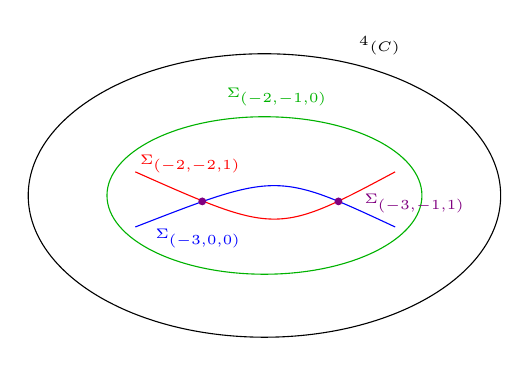
\begin{tikzpicture}
\draw [black!30!green] (3, 4+.75+1) node {\tiny $\Sigma_{(-2,-1,0)}$};
\draw (2.84,4.5) ellipse (3cm and 1.8cm);
\draw [black!30!green] (2.84,4.5) ellipse (2cm and 1cm);
\draw [red] (1.2,4.8) .. controls (3, 4) .. (4.5, 4.8);
\draw [red] (1.9, 4.9) node {\tiny $\Sigma_{(-2,-2,1)}$};
\draw [blue] (1.2,4.1) .. controls (3, 4.8) .. (4.5, 4.1);
\draw [blue] (2, 3.95) node {\tiny $\Sigma_{(-3,0, 0)}$};
\draw [violet] (2.05, 4.425) node [circle,fill,inner sep=1pt]{};
\draw [violet] (3.78, 4.425) node [circle,fill,inner sep=1pt]{};
\draw [violet] (4.75, 4.4) node {\tiny $\Sigma_{(-3, -1, 1)}$};
\draw (4.3, 6.4) node {\tiny $\Pic^4(C)$};
\end{tikzpicture}
\end{center}
We have
\[\Sigmabar_{(-1, -1, -1)}(C, f) = \Pic^4(C) \qquad \text{and} \qquad \Sigmabar_{(-2, -1, 0)}(C, f) = W^0_4(C).\]
Meanwhile, the Brill-Noether locus $W^1_4(C)$ consists of two (intersecting) components, which are distinguished by splitting type of the push forward.
 If $H$ is the trigonal class and $K$ is the canonical divisor, we have
\begin{align*}
\Sigmabar_{(-2, -2, 1)}(C, f) &= \{L \in \Pic^4(C) : h^0(C, L(-H)) \geq 1\} = \{H + p\}_{p \in C} \\
\Sigmabar_{(-3, 0, 0)}(C, f) &=  \{L \in \Pic^4(C) : h^0(C, L(H))  \geq 4\} = \{K - H - q\}_{q \in C}.
\end{align*}
We recognize these splitting types as $\vec{w}_{1,1} = (-2, -2, 1)$ and $\vec{w}_{1,0} = (-3, 0, 0)$.
Finally, the splitting locus $\Sigmabar_{(-3, -1, 1)}(C, f)$ is the intersection of the two curves above. 
If $p_0$ and $q_0$ denote the unique pair of points such that $p_0 + q_0 \sim K - 2H$, 
the intersection consists of the two points $H + p_0 \sim K - H - q_0$ and $H + q_0 \sim K - H - p_0$. This example will be revisited in Example \ref{revisit}.
\end{Example}


Our main result determines the dimensions and smoothness of all Brill-Noether splitting loci for general degree $k$ covers.
\begin{theorem}
\source{refined-brill-noether-theory-hurwitz-spaces}
\notready \label{main}
\source{refined-brill-noether-theory-hurwitz-spaces}
Let $f\colon  C \rightarrow \pp^1$ be a general degree $k$, genus $g$ cover.
Let $d$ be any integer and let $\vec{e} = (e_1, \ldots, e_k)$ be a collection of integers with $e_1 + \ldots + e_k = d - g - k + 1$.
If $u(\vec{e}) \leq g$, then $\Sigma_{\vec{e}}(C, f)$ is smooth of pure dimension $g - u(\vec{e})$. If $u(\vec{e}) > g$ then $\Sigma_{\vec{e}}(C, f)$ is empty.
\end{theorem}

The case $k = 2$ is a classical result of Clifford. (In this case, $\Sigmabar_{\vec{e}}(C, f)$ is the image of a certain symmetric power of $C$ in $\Pic^d(C)$.) We therefore assume for the rest of the paper that $k > 2$.
\begin{remark}
\source{refined-brill-noether-theory-hurwitz-spaces}
\notready
The Hurwitz space $\H_{k,g}$ is only known to be irreducible when the characteristic of the ground field is greater than $k$. If the characteristic is less than or equal to $k$, then by ``general degree $k$ cover" we shall mean a general deformation of our degeneration, so the conclusion holds for general $C \to \pp^1$ in some component of $\H_{k,g}$.
\end{remark}

\begin{remark}
\source{refined-brill-noether-theory-hurwitz-spaces}
\notready
Since it has the expected codimension, the class of $\Sigmabar_{\vec{e}}(C, f)$ is determined by the universal splitting degeneracy formulas of \cite{L}
 (see  Example \ref{revisit}).
 \end{remark}


\vspace{.1in}
\noindent
\textbf{Key ideas of the proof.}
\begin{enumerate}

\item To prove that our splitting loci are smooth of the expected dimension,
it suffices to show that for general $C$, the natural map
\[\Def^1(L) = H^1(\O_C) \rightarrow H^1(End(f_*L)) = \Def^1(f_*L)\]
is surjective for all $L \in \Pic^d(C)$.
Equivalently, by Serre duality, we seek to show that
\begin{equation} \label{sdd}
\source{refined-brill-noether-theory-hurwitz-spaces}
H^0(End(f_*L)(-p-q)) \to H^0(\omega_C)
\end{equation}
is injective, where $p, q$ are points on $\pp^1$
(whose sum gives the dualizing sheaf).

\item To accomplish this, we degenerate $C$ to a chain of elliptic curves, each mapping with degree $k$ to a chain of $\pp^1$'s.
On such reducible curves, \eqref{sdd} is \emph{not} necessarily injective.

\item To solve this problem,
we give an explicit description
of which endomorphisms of $f_* L$ deform with the curve.
We then apply this description to the kernels of \eqref{sdd} to show
that none of these sections deform with a general smoothing.

\item To show that the expected splitting loci are non-empty, we prove their expected classes are non-zero.
Using the universal splitting degeneracy formulas in \cite{L}, we prove
\[[\Sigmabar_{\vec{e}}(C, f)] = a_{\vec{e}} \theta^{u(\vec{e})},\]
where $a_{\vec{e}} \in \qq$ depends only on $\vec{e}$ \textit{and not on $g$}.
In general, the formulas for $a_{\vec{e}}$ are intractible to compute directly.
Instead, we deduce $a_{\vec{e}} \neq 0$ for $g$ sufficiently large by calculating $a_{\ee}$ for suitably chosen specialization $\ee$ of $\vec{e}$ where the formulas become simple.
\end{enumerate}
\vspace{.1in}

As a special case, Theorem \ref{main} determines the dimensions of all components of $W^r_d(C)$, thereby answering Question 1.12 of \cite{Pf}, and giving new proofs of the theorems in \cite{JR, Pf}.
\begin{Corollary}
\source{refined-brill-noether-theory-hurwitz-spaces}
\notready \label{cor}
\source{refined-brill-noether-theory-hurwitz-spaces}
Let $C$ be a general $k$-gonal curve of genus $g$. Let $\vec{w}_{r, \ell}$ denote the rank $k$, degree $d - g +k-1$ splitting type with $r+1 - \ell$ nonnegative parts that is maximal among those with $r+1$ global sections.
Every component of $W^r_d(C)$ is generically smooth of dimension $g - u(\vec{w}_{r,\ell}) = \rho(g, r - \ell, d) - \ell k $ for some $\max\{0, r + 2 - k\} \leq \ell \leq r$ such that $\ell = 0$ or $\ell \leq  g - d + 2r + 1 - k$.
Such a component exists for each $\ell$ with $g - u(\vec{w}_{r,\ell})  \geq 0$.
\end{Corollary}

In other words, splitting loci explain the different dimensions of components of $W^r_d(C)$ when $C$ is a general $k$-gonal curve. 
For example, when $f\colon  C \rightarrow \pp^1$ is a general trigonal curve of genus $6$, we have $\vec{w}_{2,1} = (-4, 0, 0)$ and $\vec{w}_{2,2} = (-3, -2, 1)$, so
\[W^1_4(C) = \Sigmabar_{(-4, 0, 0)}(C, f) \cup \Sigmabar_{(-3, -2, 1)}(C, f).\]
We have $u(-4, 0, 0) = 6$ so $\dim \Sigmabar_{(-4, 0, 0)} = 0$. This corresponds to the isolated $g^1_4$ associated to $C \subset \pp^1 \times \pp^1$ as a curve of bidegree $(3, 4)$. On the other hand, $u(-3, -2, 1) = 5$ so $\dim \Sigmabar_{(-3, -2, 1)} = 1$, corresponding to the $g^1_3$ plus any base point. 

\begin{remark}
\source{refined-brill-noether-theory-hurwitz-spaces}
\notready
Upon completing this manuscript, the author learned that Cook-Powell--Jensen have a simultaneous and independent proof that $\Sigma_{\vec{w}_{r,\ell}}(C, f)$ has a component of the expected dimension \cite{CPJ}.
\end{remark}

This paper is organized as follows. In Section \ref{split}, we recall the splitting behavior of families of vector bundles on $\pp^1$ and describe its application to Brill-Noether splitting loci. Assuming Theorem \ref{main}, Corollary \ref{cor} follows from the combinatorial structure of splitting loci stratifications. Section \ref{dimbounds} bounds the dimension of $\Sigma_{\vec{e}}(C, f)$ from above by considering a degeneration to a chain of elliptic curves. Further analysis on this degeneration yields a proof of smoothness in Section \ref{smoothness}.
 Finally, in Section \ref{existence}, we prove existence of Brill-Noether splitting loci by showing enumerative formulas for their expected classes are non-zero.


\subsection*{Acknowledgements} This work was inspired by Geoffrey Smith, who introduced the notion of Brill-Noether splitting loci in a seminar at Stanford and asked if the author's results in \cite{L} could be applied to show their existence. I am grateful for his insight. Thanks also to Ravi Vakil, Eric Larson, Sam Payne, and Melanie Wood for fruitful discussions.  I thank Kaelin Cook-Powell and Dave Jensen for their generosity and openness in sharing their work. I am grateful to the Hertz Foundation Graduate Fellowship, NSF Graduate Research Fellowship, Maryam Mirzakhani Graduate Fellowship, and the Stanford Graduate Fellowship for their generous support.
